% Created by tikzDevice version 0.12.3.1 on 2023-03-02 09:18:35
% !TEX encoding = UTF-8 Unicode
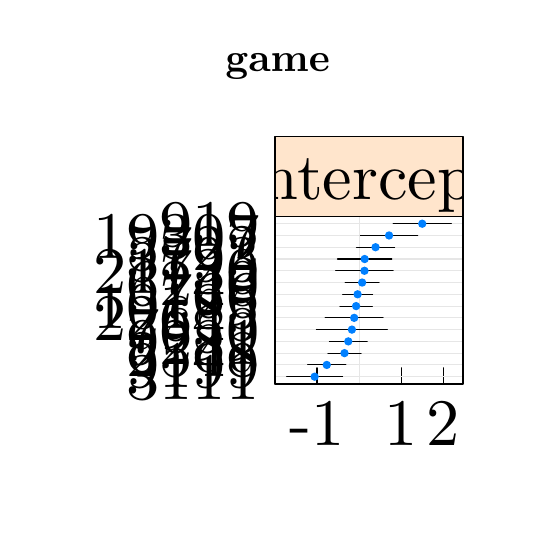
\begin{tikzpicture}[x=1pt,y=1pt]
\definecolor{fillColor}{RGB}{255,255,255}
\path[use as bounding box,fill=fillColor,fill opacity=0.00] (0,0) rectangle (180.67,180.67);
\begin{scope}
\path[clip] (  0.00,  0.00) rectangle (180.67,180.67);

\path[] (  0.00,  0.00) rectangle (180.68,180.68);
\definecolor{drawColor}{RGB}{0,0,0}

\node[text=drawColor,anchor=base,inner sep=0pt, outer sep=0pt, scale=  1.44] at ( 90.34,164.71) {\bfseries game};
\end{scope}
\begin{scope}
\path[clip] (  0.00,  0.00) rectangle (180.67,180.67);
\definecolor{drawColor}{RGB}{0,0,0}

\node[text=drawColor,anchor=base east,inner sep=0pt, outer sep=0pt, scale=  2.40] at ( 83.74, 46.29) {3111};

\node[text=drawColor,anchor=base east,inner sep=0pt, outer sep=0pt, scale=  2.40] at ( 83.74, 50.54) {9199};

\node[text=drawColor,anchor=base east,inner sep=0pt, outer sep=0pt, scale=  2.40] at ( 83.74, 54.79) {2548};

\node[text=drawColor,anchor=base east,inner sep=0pt, outer sep=0pt, scale=  2.40] at ( 83.74, 59.04) {9281};

\node[text=drawColor,anchor=base east,inner sep=0pt, outer sep=0pt, scale=  2.40] at ( 83.74, 63.30) {7650};

\node[text=drawColor,anchor=base east,inner sep=0pt, outer sep=0pt, scale=  2.40] at ( 83.74, 67.55) {22645};

\node[text=drawColor,anchor=base east,inner sep=0pt, outer sep=0pt, scale=  2.40] at ( 83.74, 71.80) {10185};

\node[text=drawColor,anchor=base east,inner sep=0pt, outer sep=0pt, scale=  2.40] at ( 83.74, 76.05) {766};

\node[text=drawColor,anchor=base east,inner sep=0pt, outer sep=0pt, scale=  2.40] at ( 83.74, 80.30) {6240};

\node[text=drawColor,anchor=base east,inner sep=0pt, outer sep=0pt, scale=  2.40] at ( 83.74, 84.56) {21730};

\node[text=drawColor,anchor=base east,inner sep=0pt, outer sep=0pt, scale=  2.40] at ( 83.74, 88.81) {3793};

\node[text=drawColor,anchor=base east,inner sep=0pt, outer sep=0pt, scale=  2.40] at ( 83.74, 93.06) {5722};

\node[text=drawColor,anchor=base east,inner sep=0pt, outer sep=0pt, scale=  2.40] at ( 83.74, 97.31) {19307};

\node[text=drawColor,anchor=base east,inner sep=0pt, outer sep=0pt, scale=  2.40] at ( 83.74,101.56) {919};
\end{scope}
\begin{scope}
\path[clip] (  0.00,  0.00) rectangle (180.67,180.67);
\definecolor{drawColor}{RGB}{0,0,0}

\path[draw=drawColor,line width= 0.6pt,line join=round,line cap=round] ( 89.46, 52.00) -- ( 89.46, 57.69);

\path[draw=drawColor,line width= 0.6pt,line join=round,line cap=round] (104.66, 52.00) -- (104.66, 57.69);

\path[draw=drawColor,line width= 0.6pt,line join=round,line cap=round] (119.85, 52.00) -- (119.85, 57.69);

\path[draw=drawColor,line width= 0.6pt,line join=round,line cap=round] (135.05, 52.00) -- (135.05, 57.69);

\path[draw=drawColor,line width= 0.6pt,line join=round,line cap=round] (150.25, 52.00) -- (150.25, 57.69);

\node[text=drawColor,anchor=base,inner sep=0pt, outer sep=0pt, scale=  2.40] at (104.66, 29.78) {-1};

\node[text=drawColor,anchor=base,inner sep=0pt, outer sep=0pt, scale=  2.40] at (135.05, 29.78) {1};

\node[text=drawColor,anchor=base,inner sep=0pt, outer sep=0pt, scale=  2.40] at (150.25, 29.78) {2};
\end{scope}
\begin{scope}
\path[clip] ( 89.43, 52.00) rectangle (157.25,112.38);
\definecolor{drawColor}{RGB}{230,230,230}

\path[draw=drawColor,line width= 0.4pt,line join=round,line cap=round] ( 89.43, 84.32) -- (157.25, 84.32);

\path[draw=drawColor,line width= 0.4pt,line join=round,line cap=round] ( 89.43,109.83) -- (157.25,109.83);

\path[draw=drawColor,line width= 0.4pt,line join=round,line cap=round] ( 89.43, 63.06) -- (157.25, 63.06);

\path[draw=drawColor,line width= 0.4pt,line join=round,line cap=round] ( 89.43, 54.55) -- (157.25, 54.55);

\path[draw=drawColor,line width= 0.4pt,line join=round,line cap=round] ( 89.43, 97.07) -- (157.25, 97.07);

\path[draw=drawColor,line width= 0.4pt,line join=round,line cap=round] ( 89.43,101.33) -- (157.25,101.33);

\path[draw=drawColor,line width= 0.4pt,line join=round,line cap=round] ( 89.43, 88.57) -- (157.25, 88.57);

\path[draw=drawColor,line width= 0.4pt,line join=round,line cap=round] ( 89.43, 71.56) -- (157.25, 71.56);

\path[draw=drawColor,line width= 0.4pt,line join=round,line cap=round] ( 89.43, 58.80) -- (157.25, 58.80);

\path[draw=drawColor,line width= 0.4pt,line join=round,line cap=round] ( 89.43, 67.31) -- (157.25, 67.31);

\path[draw=drawColor,line width= 0.4pt,line join=round,line cap=round] ( 89.43, 80.06) -- (157.25, 80.06);

\path[draw=drawColor,line width= 0.4pt,line join=round,line cap=round] ( 89.43,105.58) -- (157.25,105.58);

\path[draw=drawColor,line width= 0.4pt,line join=round,line cap=round] ( 89.43, 92.82) -- (157.25, 92.82);

\path[draw=drawColor,line width= 0.4pt,line join=round,line cap=round] ( 89.43, 75.81) -- (157.25, 75.81);

\path[draw=drawColor,line width= 0.4pt,line join=round,line cap=round] (119.85, 52.00) -- (119.85,112.38);
\definecolor{drawColor}{RGB}{0,0,0}

\path[draw=drawColor,line width= 0.4pt,line join=round,line cap=round] (113.82, 84.32) -- (124.62, 84.32);

\path[draw=drawColor,line width= 0.4pt,line join=round,line cap=round] (132.05,109.83) -- (153.08,109.83);

\path[draw=drawColor,line width= 0.4pt,line join=round,line cap=round] (108.48, 63.06) -- (120.47, 63.06);

\path[draw=drawColor,line width= 0.4pt,line join=round,line cap=round] ( 93.60, 54.55) -- (113.79, 54.55);

\path[draw=drawColor,line width= 0.4pt,line join=round,line cap=round] (111.97, 97.07) -- (131.58, 97.07);

\path[draw=drawColor,line width= 0.4pt,line join=round,line cap=round] (118.83,101.33) -- (132.57,101.33);

\path[draw=drawColor,line width= 0.4pt,line join=round,line cap=round] (114.74, 88.57) -- (126.99, 88.57);

\path[draw=drawColor,line width= 0.4pt,line join=round,line cap=round] (104.33, 71.56) -- (130.00, 71.56);

\path[draw=drawColor,line width= 0.4pt,line join=round,line cap=round] (101.16, 58.80) -- (114.99, 58.80);

\path[draw=drawColor,line width= 0.4pt,line join=round,line cap=round] (109.00, 67.31) -- (122.69, 67.31);

\path[draw=drawColor,line width= 0.4pt,line join=round,line cap=round] (112.82, 80.06) -- (124.53, 80.06);

\path[draw=drawColor,line width= 0.4pt,line join=round,line cap=round] (120.23,105.58) -- (140.94,105.58);

\path[draw=drawColor,line width= 0.4pt,line join=round,line cap=round] (111.31, 92.82) -- (132.08, 92.82);

\path[draw=drawColor,line width= 0.4pt,line join=round,line cap=round] (107.52, 75.81) -- (128.45, 75.81);
\definecolor{fillColor}{RGB}{0,128,255}

\path[fill=fillColor] (119.22, 84.32) circle (  1.51);

\path[fill=fillColor] (142.57,109.83) circle (  1.51);

\path[fill=fillColor] (114.48, 63.06) circle (  1.51);

\path[fill=fillColor] (103.69, 54.55) circle (  1.51);

\path[fill=fillColor] (121.77, 97.07) circle (  1.51);

\path[fill=fillColor] (125.70,101.33) circle (  1.51);

\path[fill=fillColor] (120.86, 88.57) circle (  1.51);

\path[fill=fillColor] (117.16, 71.56) circle (  1.51);

\path[fill=fillColor] (108.08, 58.80) circle (  1.51);

\path[fill=fillColor] (115.85, 67.31) circle (  1.51);

\path[fill=fillColor] (118.68, 80.06) circle (  1.51);

\path[fill=fillColor] (130.59,105.58) circle (  1.51);

\path[fill=fillColor] (121.70, 92.82) circle (  1.51);

\path[fill=fillColor] (117.98, 75.81) circle (  1.51);
\end{scope}
\begin{scope}
\path[clip] (  0.00,  0.00) rectangle (180.67,180.67);
\definecolor{drawColor}{RGB}{0,0,0}

\path[draw=drawColor,line width= 0.6pt,line join=round,line cap=round] ( 89.43, 52.00) rectangle (157.25,112.38);
\end{scope}
\begin{scope}
\path[clip] ( 89.43,112.38) rectangle (157.25,141.29);
\definecolor{drawColor}{RGB}{255,229,204}
\definecolor{fillColor}{RGB}{255,229,204}

\path[draw=drawColor,line width= 0.4pt,line join=round,line cap=round,fill=fillColor] ( 89.43,112.38) rectangle (157.25,141.29);
\definecolor{drawColor}{RGB}{0,0,0}

\node[text=drawColor,anchor=base west,inner sep=0pt, outer sep=0pt, scale=  2.40] at ( 66.66,118.57) {(Intercept)};
\end{scope}
\begin{scope}
\path[clip] (  0.00,  0.00) rectangle (180.67,180.67);
\definecolor{drawColor}{RGB}{0,0,0}

\path[draw=drawColor,line width= 0.6pt,line join=round,line cap=round] ( 89.43,112.38) rectangle (157.25,141.29);
\end{scope}
\end{tikzpicture}
